%!TEX root = ../../sbc-template.tex

\emph{Deep Learning} (DL), também conhecido como Aprendizado Profundo, compreende um conjunto de técnicas de Machine Learning (ML) que podem ser aplicadas em problemas de aprendizado supervisionado e não-supervisionado. A principal característica dos modelos neste domínio é a capacidade de representar e reconhecer características sucessivamente complexas, por meio da adição de níveis ou camadas de operações não-lineares em sua arquiteturas, a exemplo das redes neurais profundas, máquinas de Boltzmann profundas e fórmulas proposicionais. Modelos deste tipo ganharam popularidade ao se mostraram capazes de resolver problemas complexos com um desempenho cada vez maior \cite{bengio2009learning}.

A melhoria do desempenho de modelos de DL é decorrente do aumento recente da quantidade de dados disponíveis sobre temas complexos, aliado ao aumento da disponibilidade de recursos computacionais para executar modelos mais robustos \cite{goodfellow2016deep,deng2014deep}. Alguns dados fornecidos pela IBM reforçam esta afirmação: em $2017$ foram gerados $2,5$ quintilhões de bytes de dados por dia, e $90\%$ do volume total de dados gerados até $2017$ no mundo foi criado somente nos últimos dois anos \cite{ibm2017bigdata}. Estes fatores possibilitaram a implementação de modelos que apresentaram uma melhoria significativa na eficiência de generalização frente a modelos existentes até então, especialmente em virtude da capacidade de organizar a computação como uma composição de várias operações não-lineares (funções de ativação) e uma hierarquia de características re-utilizadas (adição de camadas) \cite{goodfellow2016deep}.
%
% Para exemplificar o efeito da adição de camadas aos modelos de DL, a Figura \ref{fig:compara_redes} mostra uma visão geral do aumento da profundidade das camadas de redes neurais e o desempenho destas em problemas de detecção de objetos em imagens. Nota-se que, à medida que a profundidade aumenta, há uma diminuição no erro. Mais recentemente, isto também tem implicado na redução do número de parâmetros treináveis, por meio da implementação de técnicas de subamostragem \cite{haykin2009neural}. Este panorama reforça a hipótese de que o aumento da profundidade das redes neurais impacta positivamente na captura de características e que estes avanços têm tornado as tarefas mais factíveis, com uma diminuição do esforço computacional associado, em comparação com modelos mais rasos \cite{goodfellow2016deep}.
%
% \begin{figure}[ht]
% 	\centering
% 	\caption{Evolução de profunidade, taxa de erro e número de parâmetros das redes neurais profundas com o passar dos anos. Fonte: \cite{mediumcnn}.}
% 	\label{fig:compara_redes}
% 	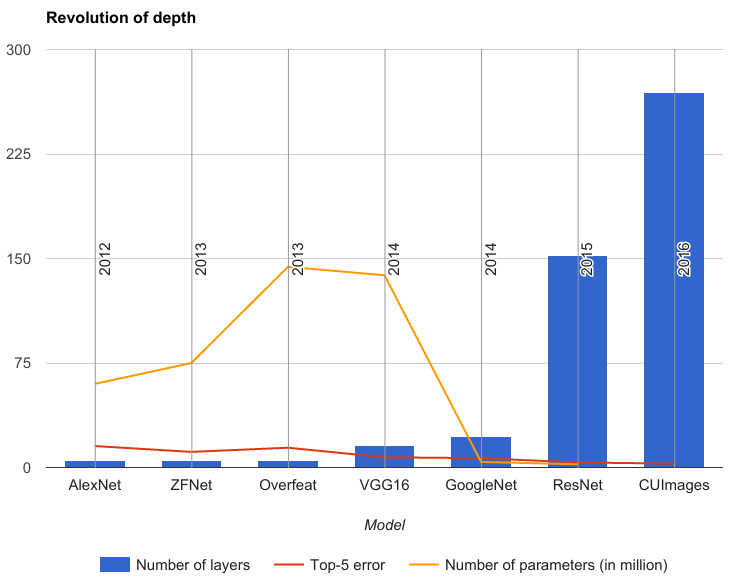
\includegraphics[width=0.8\textwidth]{img/compara_redes.png}
% \end{figure}

% \subsection{Breve Histórico}
%
% O termo \emph{Deep Learning} (DL) não é recente, foi utilizado pela primeira vez por Dechter, no contexto da descoberta de todas as configurações de conflitos mínimas a fim de resolver um problema de satisfação de restrições \cite{dechter1986learning}. Porém, ganhou força a partir de pesquisas sobre RNAs \emph{feedforward} com muitas camadas ocultas, também conhecidas por redes neurais profundas \cite{deng2014deep}.
%
% Considera-se que o desenvolvimento de DL pode ser dividido em três momentos. No primeiro momento, houve a proposição de modelos lineares simples, compostos apenas por um neurônio, a exemplo dos neurônios de McCulloch e Pitts \cite{mcculloch1943logical} e \emph{Perceptron} de Rosenblatt  \cite{rosenblatt1958perceptron}. No segundo instante, iniciado nos anos 1980, teve-se como eixo central a interconexão entre vários neurônios e a proposição do algoritmo \emph{back-propagation} para ajuste de pesos no treinamento das RNAs \cite{rumelhart1986parallel,rumelhart1986backpropagation}. Com estas contribuições, houve aplicação das RNAs em diversos domínios. Ainda no final deste segundo momento, duas contribuições relevantes foram feitas: os modelos \emph{Long Short-Term Memory} (LSTM) e LeNet. Esta última utiliza o algoritmo de \emph{backpropagation} para treinar uma rede neural convolucional profunda para reconhecer dígitos escritos à mão \cite{lenet}.
%
% A terceira fase tem um marco inicial definido: compreende o ano de $2006$, quando Hinton utilizou o termo \emph{deep belief network} para designar um tipo de modelo de RNA MLP cujo treinamento adota uma estratégia gulosa e orientada a camadas. Cada camada é pré-treinada individualmente como uma máquina de Boltzmann restrita, e o modelo inteiro é então ajustado utilizando técnicas de treinamento supervisionado, incluindo o algoritmo de \emph{backpropagation}. A partir deste marco, outros pesquisadores passaram a investigar a técnica de Hinton e, com o tempo, o termo \emph{deep learning} passou a designar modelos compostos de várias camadas sucessivas de operações não lineares utilizados para o aprendizado de determinada tarefa \cite{hinton2006fast, hinton2007learning, goodfellow2016deep, deng2014deep}.
%
% Na conjectura atual, modelos de DL têm superado significativamente o estado da arte de modelos inteligentes em diversas competições em todo o mundo. A \emph{ImageNet Large Scale Visual Recognition Challenge} (ILSVRC) \cite{ImagenetChall} é uma competição em que equipes de pesquisa avaliam seus algoritmos em um conjunto de dados fornecido, e competem para chegar à melhor acurácia em várias tarefas de reconhecimento visual automático. O conjunto de dados utilizado, denominado ImageNet \cite{Imagenet:main}, consiste de um conjunto de aproximadamente $14$ milhões de imagens de $21$ mil categorias organizadas hierarquicamente, em que cada uma contém algumas centenas de imagens de exemplo. A performance dos modelos submetidos para a competição é chamada taxa de erro top-5, e representa o erro computado quando a classe alvo não se encontra entre as 5 apontadas pelo modelo como as que têm maior probabilidade de estarem na imagem. Em 2011, os melhores resultados de  classificação no ILSVRC tinham por volta de $25\%$ de erro top-5 nas tarefas propostas. Em 2012, o modelo AlexNet, uma rede neural convolucional proposta segundo as ideias de DL, atingiu apenas $16,4\%$ de erro, propondo um ganho até então nunca visto entre duas edições sucessivas da competição \cite{ImagenetChall:2012}.
%
% O gráfico da Figura \ref{fig:compara_redes} sintetiza o histórico da competição ILSVRC, em que a partir do ano de 2012 houve a introdução de modelos baseados em DL. O histograma mostra a diminuição do erro na tarefa de aprendizado proposta e a linha tracejada enfatiza o número de camadas ocultas utilizadas nos modelos vencedores.
%
% \begin{figure}[ht]
% 	\centering
% 	\caption{Evolução do erro dos modelos vencedores da competição ILSVRC pela profundidade das redes neurais \cite{dl_ILSVRC, ImagenetChall}}
% 	\label{fig:compara_redes_ilsvrc}
% 	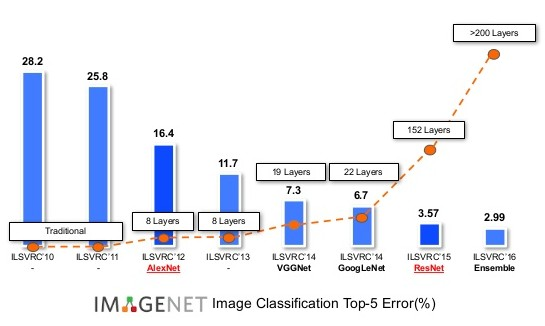
\includegraphics[width=0.8\textwidth]{img/compara_redes_ilsvrc.png}
% \end{figure}
%
% Apesar do foco inicial de DL ter sido concentrado no desenvolvimento de técnicas de aprendizado não-supervisionado e na habilidade de modelos profundos de boa generalização a partir de conjuntos de dados pequenos, o cenário atual das pesquisas nesta área consideram o uso de técnicas de aprendizado supervisionado visando o endereçamento de conjuntos de dados massivos e categorizados, e também redes neurais profundas híbridas, que misturem técnicas e conceitos de diferentes origens \cite{deng2014deep,goodfellow2016deep}.
%
% Dentre estes resultados de vanguarda no ILSVRC destacam-se os modelos de DL construídos com redes neurais convolucionais, que têm impulsionado os mais recentes avanços na área de Visão Computacional desde a proposição na literatura da rede LeNet \cite{lenet}. Em particular, desde a proposição e vitória do modelo AlexNet \cite{alexnet} no ano de 2012, as redes neurais convolucionais têm dominado o ranking dos anos seguintes da competição, conforme ilustrado na Figura \ref{fig:compara_redes_ilsvrc} \cite{deng2014deep}. Dada a importância deste tipo de rede neural, os conceitos sobre as mesmas e os modelos canônicos serão apresentados a seguir.


\subsection{Redes Neurais Convolucionais} \label{subsubsec:rnc}
%!TEX root = ../../sbc-template.tex
\emph{Redes Neurais Convolucionais} (CNNs, do inglês \emph{Convolutional Neural Networks}) são uma classe de redes neurais \emph{feedforward} com topologia bem definida e estrutura em grade, com o uso de operações de convolução em pelo menos uma de suas camadas \cite{goodfellow2016deep}. Aplicadas em tarefas de classificação, regressão, localização, detecção e outras, este tipo de modelo se destaca no reconhecimento de padrões em dados de alta dimensionalidade, a exemplo de séries temporais, imagens e vídeos \cite{Khan:Livro}.

A operação de convolução possui um papel central nas CNNs. Esta operação descreve a média ponderada de uma determinada função $x_1(t)$ sob um intervalo fixo de uma variável, enquanto os pesos da média ponderada considerada pertencem à função $x_2(t)$ amostrados em intervalos $a$ \cite{bracewell1986fourier}. Assim, a convolução $s(t)$ de duas funções $x_1(t)$ e $x_2(t)$ é uma função $s: \mathds{Z} \rightarrow \mathds{R}$, denotada $s(t) = x_1(t) * x_2(t)$, e definida conforme Equação \ref{eq:int_convolucao} \cite{lathi2006sinais}:

\begin{equation}\label{eq:int_convolucao}
s(t) = x_1(t) * x_2(t) = \int_{-\infty}^{\infty} x_1(a) x_2(t-a)da.
\end{equation}

No contexto de ML, a função $x_1(t)$ é chamada de \emph{input}, a função $x_2(t)$ é o \emph{kernel}, e a saída $s(t)$ consiste no \emph{feature map}, ou mapa de características. No contexto prático, o \emph{input} normalmente é um vetor multidimensional de dados e o \emph{kernel} é um vetor multidimensional de pesos que devem ser ajustados para aprendizado das CNN. Considerando, por exemplo, uma imagem $I$ de dimensões $(m,n)$ como \emph{input} e a aplicação de um \emph{kernel} $K$, a versão discreta da convolução, passível de implementação computacional e equivalente à Equação \ref{eq:int_convolucao}, é mostrada na Equação \ref{eq:conv_img}:
\begin{equation}
 S(i,j) = I(i,j)*K(i,j) = \sum_{m}\sum_{n}I(m,n)K(i-m,j-n),\label{eq:conv_img}
\end{equation}
em que $S$ é o \emph{feature map} resultante e $(i,j)$ é a posição correspondente nesse mapa. Para otimizar os aspectos de implementação, os valores resultantes da operação de convolução são armazenados apenas nas posições $(i,j)$ explicitamente declaradas \cite{goodfellow2016deep}.

Os \emph{feature maps}, resultantes das operações de convolução, compreendem a noção de filtros, responsáveis por capturarem características relativas à entrada, tais como contornos, linhas, texturas, etc. Quando combinados de maneira sequencial, como proposto pelas CNNs, as características capturadas pelas camadas convolucionais vão se tornando mais complexas à medida que se aumenta a profundidade da rede. Assim, um primeiro \emph{feature map} de uma camada convolucional captura um simples contorno, enquanto um \emph{feature map} em uma camada mais profunda da rede pode capturar uma forma, um rosto ou até um objeto inteiro \cite{Buduma:Livro}. Esta noção é ilustrada na Figura \ref{fig:convolutions}.

\begin{figure}[!h]
	\centering
	\caption{Papel das camadas convolucionais e \emph{feature maps} nas CNNs. Fonte: \cite{Khan:Livro}.}
	\label{fig:convolutions}
	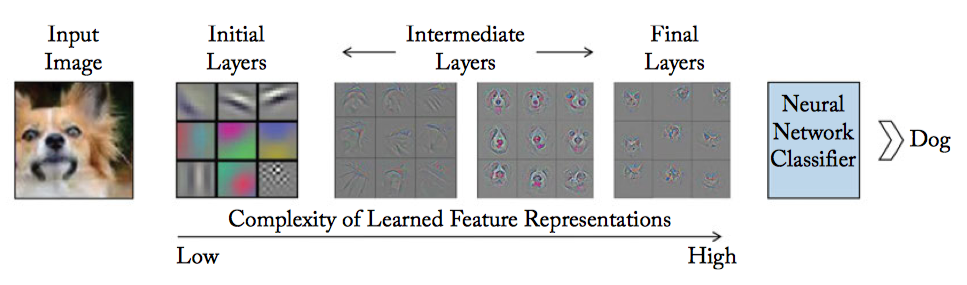
\includegraphics[width=0.8\textwidth]{./img/fundamenta/convolutions}
\end{figure}

As camadas convolucionais, que capturam os \emph{feature maps} e contém os pesos da rede, normalmente são seguidas por funções de ativação como as exemplificadas na Seção \ref{sec:rnas}, mais especificamente na Tabela \ref{tab:ativacoes}. Via de regra, a toda camada convolucional em uma CNN, segue-se uma função de ativação, finalizando em uma operação de \emph{pooling}, como mostra a Figura \ref{fig:cnn_camada}.

\begin{figure}
	\centering
	\caption{Componentes de uma camada de uma rede neural convolucional \cite{goodfellow2016deep}.}
	\label{fig:cnn_camada}
	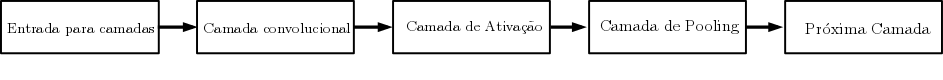
\includegraphics[width=\textwidth]{img/cnn_camada_ipe.png}
\end{figure}

 Uma função de \emph{pooling} substitui a saída da rede em determinada localização por uma síntese estatística das saídas vizinhas. Por exemplo, a operação \emph{max pooling} retorna o valor máximo em uma área retangular, enquanto a \emph{average pooling} retorna a média das saídas de um retângulo. O objetivo desta operação é fazer com que o \emph{feature map} seja invariante a pequenas mudanças na entrada. Esta invariância à pequenas mudanças locais é uma propriedade útil quando o mais importante for a existência da característica e não exatamente a sua posição, o que aumenta a eficiência geral da CNN ao reduzir drasticamente o número de valores a serem passados entre duas camadas quaisquer \cite{goodfellow2016deep}.

 Outros parâmetros, como \emph{padding} e \emph{strides}, são importantes para a captura de características. O parâmetro \emph{padding} consiste em adicionar um número de linhas e colunas em cada lado da entrada de maneira a controlar o tamanho do \emph{feature map} resultante da operação de convolução. Já a distância entre duas janelas da convolução, ou da operação de \emph{pooling}, é medida através do número de \emph{strides}. Ambos parâmetros manipulam as dimensões das saídas das camadas de uma CNN \cite{chollet2017deep}.

Embora se tenha uma noção clara das camadas individuais e de suas respectivas funções, a combinação das mesmas em uma rede neural convolucional não é uma tarefa trivial, podendo resultar em um número arbitrariamente grande de redes com milhares de parâmetros ajustáveis, cujo desempenho acerca de um problema ainda precisará ser aferido. Considerando os esforços computacionais para isto, a maioria das soluções atuais baseadas em DL fazem uso de CNNs canônicas já propostas na literatura, as quais são apresentadas a seguir.


% \subsection{Modelos Canônicos de Redes Neurais Convolucionais} \label{subsubsec:modelos_canonicos}
% %!TEX root = ../../sbc-template.tex

Os modelos canônicos de CNNs são arquiteturas que trouxeram contribuições importantes, pioneiras na aplicação de técnicas que são comuns ainda hoje no cenário de DL, comumente utilizadas em diversas tarefas de aprendizado \cite{9dlpapers}.

A LeNet é o primeiro modelo de rede neural a aplicar convoluções ao invés das camadas totalmente conectadas convencionais. Foi proposta por LeCun em 1998 e é composta de 7 camadas, sendo uma camada de entrada, duas camadas convolucionais, duas camadas de \emph{pooling}, uma camada totalmente conectada e a camada de saída. A tarefa de aprendizado endereçada por esta rede na ocasião de sua proposição foi o reconhecimento de dígitos manuscritos. Para o treinamento e teste desta rede foi utilizado o conjunto de dados \emph{Modified National Institute of Standards and Technology} (MNIST), composto de 60000 imagens de treinamento e 10000 de teste dos dígitos de 0 a 9 escritos à mão \cite{mnist}. A LeNet foi amplamente utilizada por bancos para o reconhecimento de números escritos à mão em cheques digitalizado em imagens em escala de cinza de tamanho $32 \times 32$ \cite{lenet}. Apesar de pesquisas nesta área continuarem no decorrer dos anos, a quantidade insuficiente de bases de imagens catalogadas e o baixo poder computacional da época fizeram com que as CNNs permanecessem sem grandes destaques até o ano de 2012 \cite{9dlpapers}.

AlexNet foi a primeira CNN ganhadora do desafio ILSVRC, em 2012, ao atingir um erro top-5 igual a $15.4\%$. O segundo melhor modelo daquele ano atingiu um erro de $26.2\%$. Esta rede, treinada para uma tarefa de classificação utilizando imagens de 1000 categorias da ImageNet, é formada por 5 camadas convolucionais com filtros de tamanho $11 \times 11$, intercaladas com camadas de \emph{max-pooling} e \emph{dropout} e $3$ camadas totalmente conectadas. Utilizava a função de ativação \emph{ReLU} ao invés da tradicional tangente hiperbólica. Na ocasião, para obter uma quantidade de exemplos razoável mediante o número de parâmetros ajustáveis, foi realizado um aumento artificial nas imagens de entrada, modificando-as segundo translações, reflexões horizontais e cortes. A AlexNet foi então treinada utilizando duas GPU GTX 580 por 5 a 6 dias, com o algoritmo de \emph{backpropagation} utilizando gradiente descendente estocástico para \emph{batch} e técnicas como \emph{momentum} e \emph{weight decay}. Estas técnicas garantiram à rede um desempenho significativamente melhor que o dos modelos tradicionais que estavam sendo aplicados para a ILSVRC daquele ano \cite{alexnet}.

Uma CNN que com um amplo destaque pela simplicidade e profundidade é a VGG. Apesar de não ter ganhado a ILSVRC 2014, alcançou um erro top-5 de $7.3\%$. Foi concebida na Universidade de Oxford, a VGG-19 contendo 19 camadas que utiliza estritamente filtros de $3 \times 3$ com \emph{stride} e \emph{pad} de 1, juntamente com \emph{max-pooling} de tamanho $2 \times 2$ e \emph{stride} 2. O número de filtros dobra após cada camada de \emph{max-pooling}, o que reforça a idéia de diminuir dimensões espaciais de largura e altura e aumentar a profundidade. A VGG-19 foi treinada em parte da base ImageNet utilizando 4 GPUs Nvidia Titan Black por duas a três semanas \cite{vggnet}.

Uma das primeiras arquiteturas de CNNs que se desviou do caminho normal de simplesmente empilhar camadas convolucionais e de pooling em uma estrutura sequencial foi a GoogLeNet, também chamada de Inception. Dotada de 22 camadas convolucionais, a rede ganhou o ILSVRC 2014 com um erro top-5 de $6.7\%$. Esta performance se deve aos chamados de módulos Inception, compostos de camadas da rede que ocorrem em paralelo. Ao invés de realizar uma operação de convolução ou \emph{max-pooling} de cada vez, várias operações diferentes são realizadas e os mapas de características obtidos são condensados e conectados ao próximo bloco Inception. A Figura \ref{fig:bloco_inception} mostra que há 4 conjuntos de operações a serem realizadas, todas contendo convoluções com filtros $1 \times 1$, podendo haver também a convolução com filtros de tamanho $3 \times 3$, $5 \times 5$, ou uma operação de \emph{max-pooling} de $3\times 3$. A convolução com filtro $1\times 1$ é aplicada para reduzir a dimensionalidade do problema reduzindo a profundidade do mapa de características, além de retirar da entrada informações bem detalhadas em volume. As convoluções que utilizam filtros de $3\times 3$ e $5\times 5$ dão ao modelo a capacidade de extrair informações relevantes em larga escala. A camada de \emph{max-pooling} é aplicada a fim de reduzir a largura e altura do mapa de característas e combater \emph{overfitting}. Na GoogLeNet, as camadas totalmente conectadas são substituídas por \emph{average pooling}, o que economiza um grande número de parâmetros. A rede, que foi treinada em algumas GPUs de alta performance por uma semana, utiliza ReLU como função de ativação e dispõe de 9 módulos Inception com mais de 100 camadas no total. Todas estas técnicas utilizadas para reduzir a dimensionalidade do problema surtiram efeito pois, como mostrado na Figura \ref{fig:compara_redes}, nota-se que esta rede tem 12 vezes menos parâmetros que a sua predecessora AlexNet \cite{inception}.

\begin{figure}[h!]
	\centering
	\caption{Bloco Inception da CNN GoogLeNet. Fonte: \cite{9dlpapers}.}
	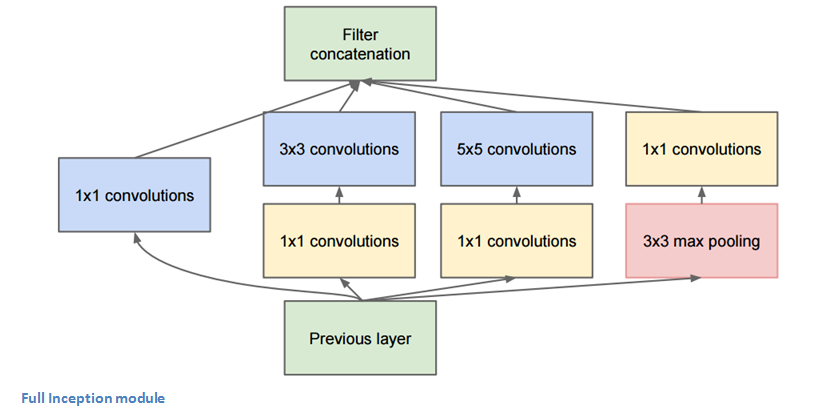
\includegraphics[width=0.7\linewidth]{img/GoogLeNet}
	\label{fig:bloco_inception}
\end{figure}

A Microsoft ResNet foi a CNN vencedora do ILSVRC 2015, com uma taxa de erro top-5 de $3.6\%$. Composta de um total de 152 camadas, esta rede neural deve o sucesso de sua profundidade ao bloco residual, representado na Figura \ref{fig:bloco_residual} que, de maneira resumida, soma à saída de um certo bloco de convoluções a saída de um bloco anterior, para que ambos \emph{feature maps} sejam alimentados à função de ativação ReLU.

\begin{figure}[h!]
\centering
\caption{Bloco Residual da CNN ResNet. Fonte: \cite{torch:resnet}.}\label{fig:bloco_residual}
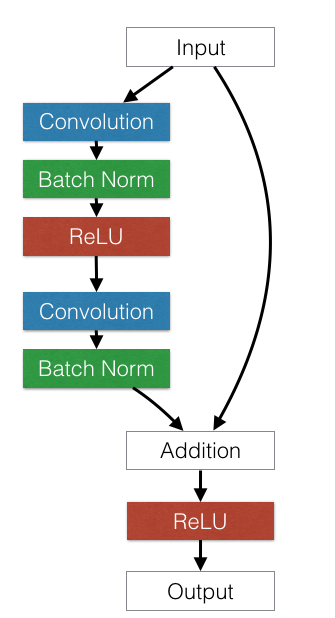
\includegraphics[height=0.3\textheight]{img/resnets_modelvariants}
\end{figure}

Em CNNs tradicionais, a partir de uma imagem de entrada, obtém-se o \emph{feature map} resultante de uma operação de convolução e então aplica-se o \emph{max-pooling}. Este resultado produz uma nova representação, que possui pouca relação com a entrada original. No caso da ResNet, o bloco residual faz com que a entrada original persista em camadas mais profundas da rede, o que garante que as características determinantes para a tarefa de aprendizado sejam disseminadas para camadas mais profundas, ao mesmo tempo em que mantém a dimensionalidade reduzida. Outra razão para o bloco residual ser efetivo é que durante a fase \emph{backwards} o gradiente vai fluir mais facilmente pela rede, pois os blocos residuais estão diretamente conectados às camadas mais rasas na arquitetura, o que facilita a distribuição do gradiente. Na ocasião da sua proposição, a ResNet foi treinada em 8 GPUs por duas a três semanas \cite{resnet}.

Observada a importância das CNNs apresentadas nesta seção, vale notar o esforço computacional para o treino das mesmas, que demora dias mesmo com um hardware específico para este fim. Todo o resultado do treinamento destas redes com o conjunto de dados ImageNet encontram-se disponíveis em \emph{frameworks} para implementação de CNNs, como o  \emph{Keras} \cite{keras:applications} e \emph{Tensorflow} \cite{tensorflow:models}. Disponibilizar estas versões de tais CNNs favorece o aproveitamento das mesmas em contextos análogos, como mostrado a seguir.

%
% \subsection{\emph{Transfer Learning}}
% %!TEX root = ../../sbc-template.tex
As várias redes convolucionais treinadas com milhares de exemplos da base de dados  ImageNet e validadas na competição ILSVRC, a exemplo das que foram mencionadas na seção anterior, registram alto desempenho nas tarefas de aprendizado para as quais foram originalmente projetadas. Considerando a arquitetura das mesmas, percebe-se como resultado do treinamento efetuado que uma grande quantidade de parâmetros foi ajustada mediante os milhares de exemplos apresentados, processo este que demorou vários dias mesmo mediante uso de hardware altamente especializado.

Segundo Oquab, representações de imagens aprendidas por CNNs a partir de conjuntos de dados com grande número de exemplos podem ser transferidas eficientemente para outras tarefas de reconhecimento visual que tenham uma quantidade limitada de dados de treinamento \cite{oquab2014learning}. Para tanto, faz-se uso de uma técnica denominada \emph{transfer learning}, que consiste em transferir os conhecimentos entre domínios relacionados. No contexto das CNNs aplicadas em reconhecimento de objetos em imagens, as camadas internas podem agir como detectores de características em médio nível. Estas podem ser pré-treinados na tarefa fonte, na qual utiliza-se um conjunto de dados vasto como o ImageNet, e então re-utilizados na tarefa alvo, que pode conter um conjunto de dados mais restrito.

Após o treinamento para a tarefa original, a rede aprendeu a identificar características mais elementares, como linhas, contornos e objetos, as quais que podem ser redirecionadas na tarefa alvo que possui um objetivo mais específico. O trabalho de Zeiler e Rob, por exemplo, ilustra uma aplicação de \emph{transfer learning}, em que os autores transferem o conhecimento de uma CNN AlexNet treinada originalmente para o conjunto de dados ImageNet adaptando-a para o conjunto de dados Caltech-256, em que a base de dados da tarefa alvo possui apenas cerca de 30 mil imagens a serem usadas numa tarefa de classificação \cite{zeiler2014visualizing}.

Na prática, o \emph{transfer learinng} é feito ao transferir os parâmetros de peso $w$ e de bias $b$ de um modelo já consolidado na literatura e pré-treinado com um conjunto de dados mais robusto, para um modelo similar ainda não treinado. Com o objetivo aproveitar os parâmetros pré-treinados, remove-se a última camada, ou seja, a camada de saída, e em seguida adiciona-se uma ou mais camadas novas, sem treinamento. Neste ponto, outros hiperparâmetros são considerados (número de camadas removidas, quantidade e tipo de camadas adicionadas, por exemplo) e o modelo passa por um processo de ajuste, chamado \emph{fine tuning}, para que ajustar os nossos parâmetros adicionados em conformidade com os pré-existentes, permitindo a extração das características do conjunto de dados da tarefa alvo de maneira satisfatória \cite{oquab2014learning}.

